\documentclass[crop,tikz]{standalone} 
\usepackage{tikz, amsmath, amssymb, graphicx} 

\DeclareMathAlphabet\mathbfcal{OMS}{cmsy}{b}{n}

\newcommand{\Mt}{\mathbfcal{M}}
\newcommand{\Yt}{\mathbfcal{Y}}
\newcommand{\Ft}{\mathbfcal{F}}

\usetikzlibrary{positioning, shapes.geometric} 

\begin{document} 

\begin{tikzpicture}


\node[inner sep=0pt] (sim:0.05) at (0,0) {
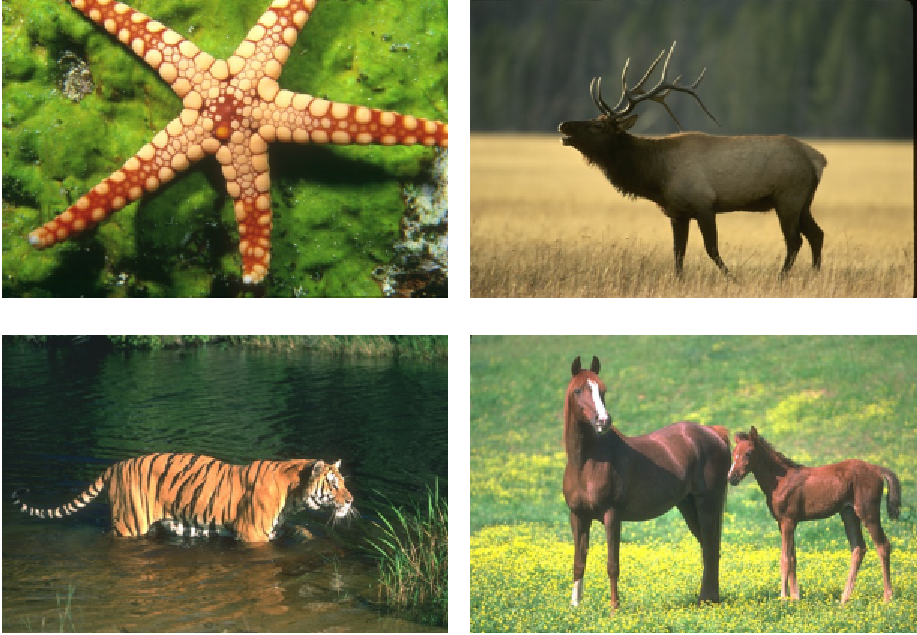
\includegraphics[width=0.6\textwidth]{images.pdf}
};

\node[inner sep=0pt] (sim:0.05) at (8,0) {
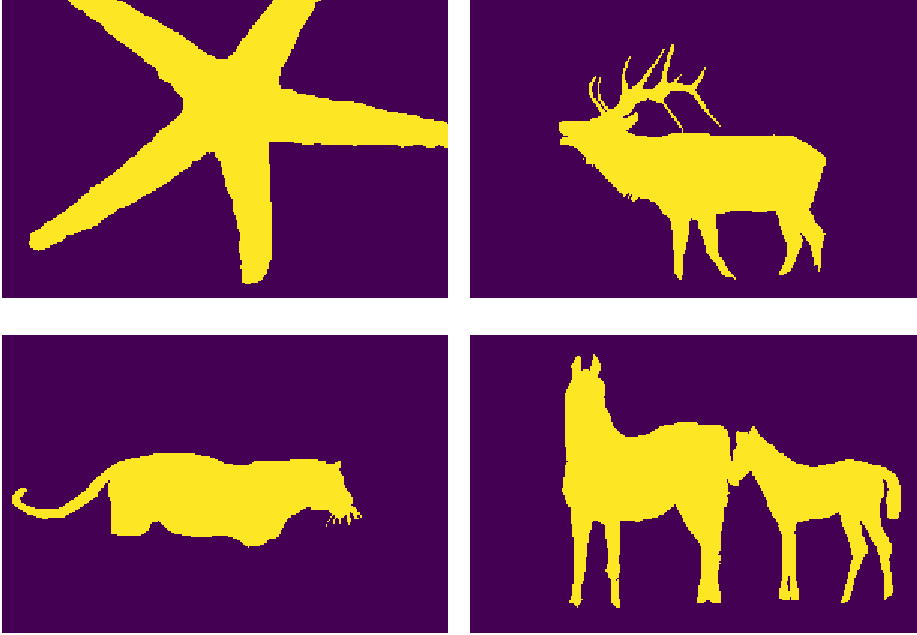
\includegraphics[width=0.6\textwidth]{ground_truths.pdf}
};


\draw (0, 3.0) node {Input Images};
\draw (8, 3.0) node {Ground Truth};




\end{tikzpicture}
\end{document} 
